\documentclass{standalone}
\usepackage{pgfplots}
\pgfplotsset{compat=newest}

\begin{document}
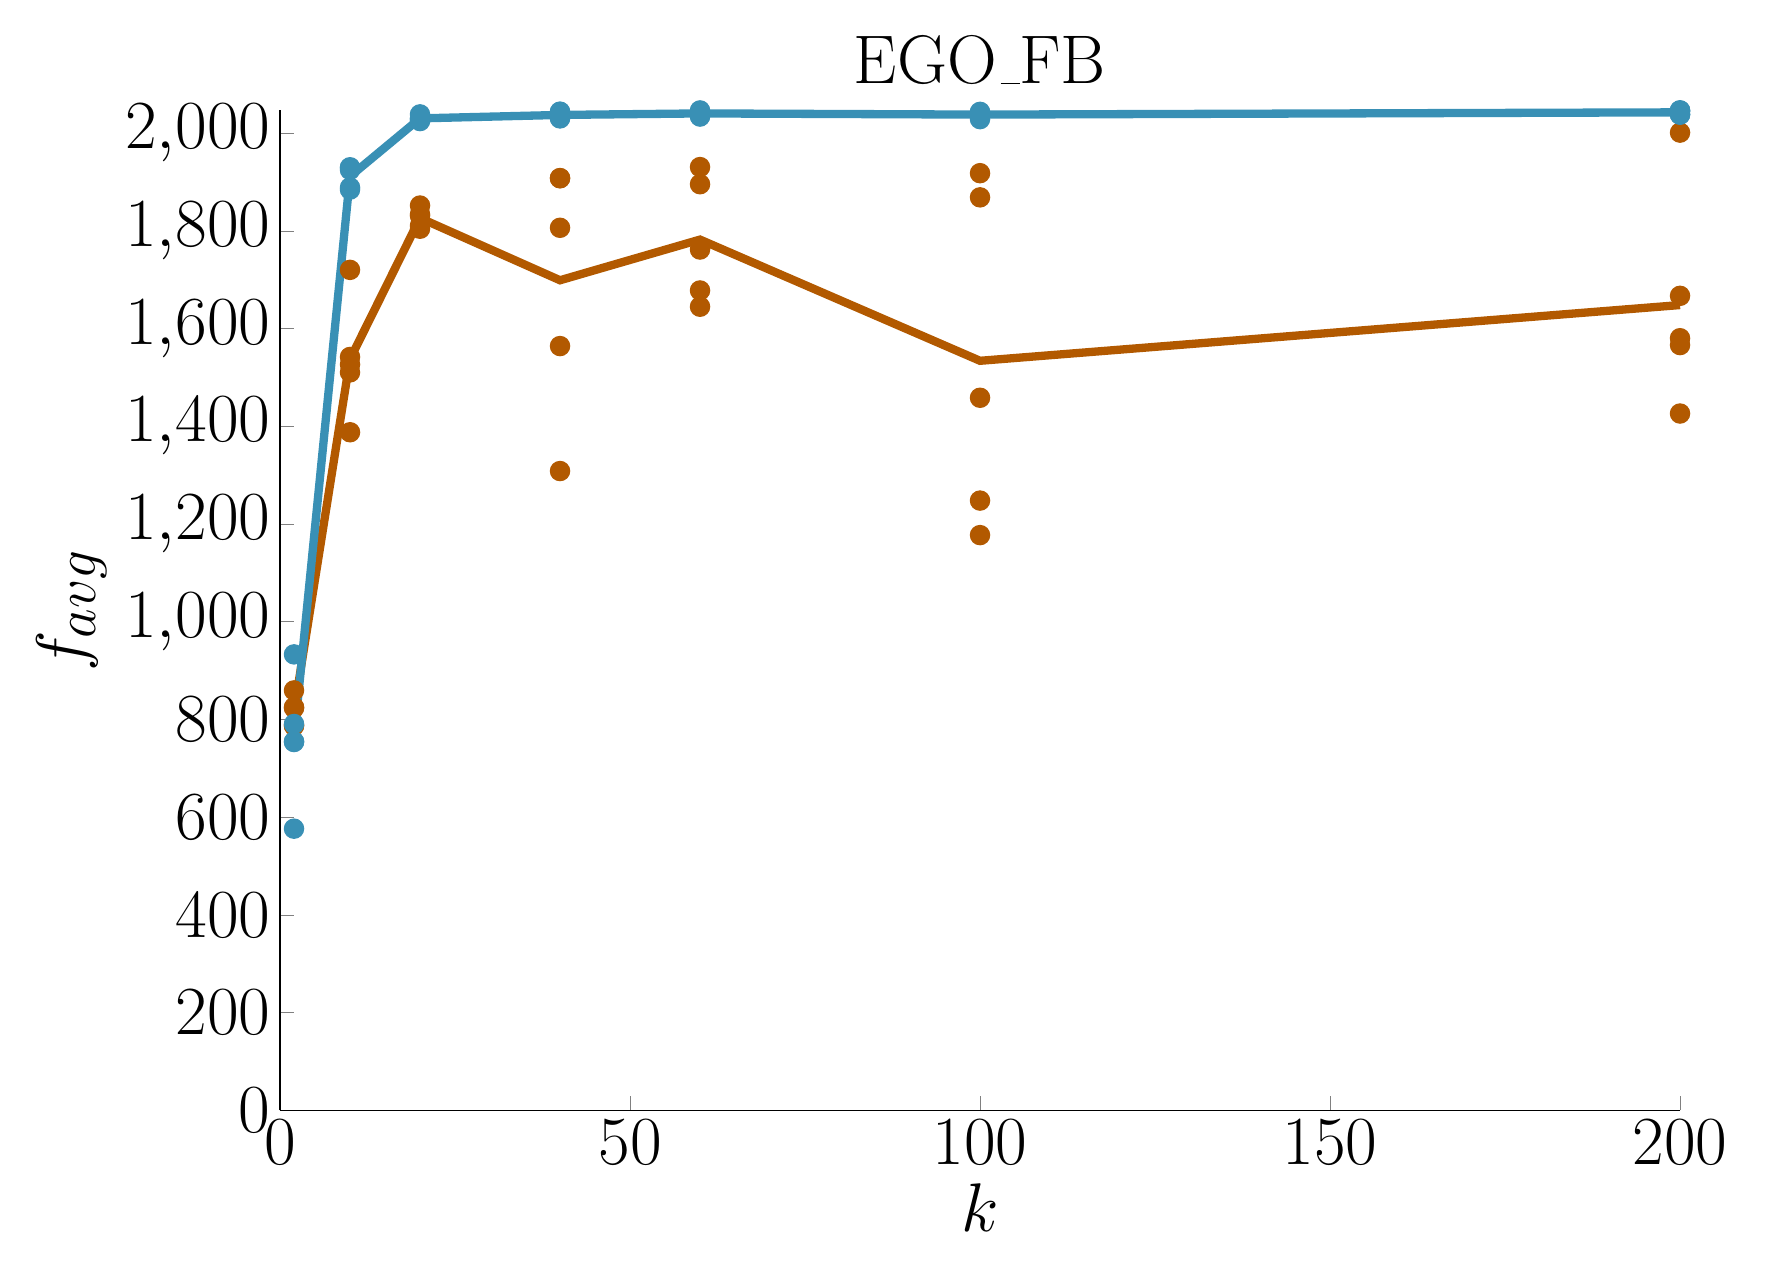
\begin{tikzpicture}

\begin{axis}[%
title style={font=\Huge},
title=EGO\_FB,
tick label style={font=\Huge},
label style={font=\Huge},
legend style={font=\Huge},
view={0}{90},
max space between ticks=50pt,
width=7in,
height=5in,
scale only axis,
xmin=0, xmax=200,
xtick={0, 50, 100, 150, 200},
xlabel={$k$},
ymin=0, ymax=2046.65,
%ytick={0, 200, 400, 600, 800, 1000},
ylabel={$f_{avg}$},
major tick length=5pt,
axis lines*=left,
legend cell align=left,
clip=false]

\addplot [
only marks,
mark=*,
mark size=3.5pt,
color=orange!70!black,
%solid,
%line width=2pt,
]
coordinates{
(2,786.85)(2,787.95)(2,823.4)(2,825.05)(2,859.4)(10,1387.75)(10,1510.3)(10,1526.35)(10,1541.8)(10,1720.1)(20,1804.25)(20,1810.6)(20,1830.65)(20,1833.6)(20,1851.75)(40,1308.35)(40,1564.15)(40,1806.2)(40,1907.5)(40,1907.95)(60,1644.65)(60,1677.95)(60,1761.7)(60,1895.4)(60,1930.45)(100,1177.25)(100,1247.9)(100,1458.35)(100,1868.5)(100,1917.95)(200,1426.1)(200,1566.15)(200,1580.2)(200,1666.95)(200,2001.0)
};

\addplot [
only marks,
mark=*,
mark size=3.5pt,
color=cyan!70!black,
%solid,
%line width=2pt,
]
coordinates{
(2,576.4)(2,753.75)(2,754.85)(2,790.65)(2,933.1)(10,1884.35)(10,1888.75)(10,1924.55)(10,1928.7)(10,1930.1)(20,2024.6)(20,2027.8)(20,2029.0)(20,2031.0)(20,2038.3)(40,2030.0)(40,2031.5)(40,2037.7)(40,2042.8)(40,2043.95)(60,2033.85)(60,2035.8)(60,2041.65)(60,2043.6)(60,2046.4)(100,2028.55)(100,2037.6)(100,2037.9)(100,2041.85)(100,2043.5)(200,2037.85)(200,2037.85)(200,2044.0)(200,2046.1)(200,2046.65)
};

\addplot [
color=orange!70!black,
solid,
line width=3pt
]
coordinates{
(2,816.53)(10,1537.26)(20,1826.17)(40,1698.83)(60,1782.03)(100,1533.99)(200,1648.08)
};

\addplot [
color=cyan!70!black,
solid,
line width=3pt
]
coordinates{
(2,761.75)(10,1911.29)(20,2030.14)(40,2037.19)(60,2040.26)(100,2037.88)(200,2042.49)
};


\end{axis}
\end{tikzpicture}
\end{document}
